\subsection{Analytic Solution To The Diffusion Equation With Reaction At The Interface}
\label{sec:analytic-diffusion-reaction}

In this section we compute the analytic solution to the diffusion equation, subject to a chemical reaction at the interface ($x = 0$).
We need to solve the equation

\begin{align}
	\frac{\partial C}{\partial t} = D\frac{\partial^2 C}{\partial x^2},
\end{align}

which must meet the border conditions

\begin{align}
	C(x = \delta, t) = C_b,\\
	-D\frac{\partial C(x = 0, t)}{\partial x} = -r,
\end{align}

and the initial condition

\begin{align}
	C(x, t = 0) = 0.
\end{align}

First, we will compute the steady state solution, that is

\begin{align}
	\frac{\partial C_{SS}}{\partial t} = 0.
\end{align}

Which, from \ref{eq:diffusion-only} takes the form

\begin{align}
	C_{SS}(x) = Ax+B,
\end{align}

where $A$ and $B$ are constants to be determined. From border conditions \ref{eq:border-conditions-reaction-diffusion},
\begin{align}
	A = \frac{r}{D},\\
	B = C_b - \frac{r\delta}{D},
\end{align}

Also, we want to take our system to the dimensionless parameters $\xi = x/\delta$ and $\tau = D t / \delta^2$, thus

\begin{align}
	C_{SS}(x) = C_b - \frac{r\delta}{D}(1-\xi).
\end{align}

The complete system including time difference can be easily treated making the non-homogenous border condition at $x=0$ homogenous. Consider the following function

\begin{align}
	\rho(\xi, \tau) = \frac{C(\xi,\tau)-C_{SS}(\xi, \tau)}{C_b}.
\end{align}

Since border conditions are met for all time, we get that 

\begin{align}
	\rho(\xi = 1, \tau) = \frac{C(\xi=1,\tau)-C_{SS}(\xi=1, \tau)}{C_b} = \frac{C_b - C_b}{C_b} = 0,\\
	-D\frac{\partial \rho(\xi = 0, \tau)}{\partial x} = \frac{-D\frac{\partial C(\xi=0,\tau)}{\partial x}+D\frac{\partial C_{SS}(\xi=1, \tau)}{\partial x}}{C_b} = \frac{-r + r}{C_b}=0.\\
\end{align}


Thus we need to solve a system with homogenous border conditions,

\begin{align}
	\frac{\partial \rho}{\partial \tau} = D\frac{\partial^2 \rho}{\partial \xi^2},
\end{align}

\begin{align}
	\rho(\xi = 1, \tau) &= 0, \\
	\frac{\partial\rho(\xi = 0, \tau)}{\partial \tau} &= 0, \\
	\rho(\xi, \tau = 0) &= -\frac{\partial C_{SS}(x)}{C_b}.
	\label{eq:initial-b-conditions}
\end{align}

This system is solve on a similar fashion as \ref{eq:diffusion-1d}: using separation of variables to obtain the solution as a Fourier series. The general solution is of the form

\begin{align}
	\rho(\xi, \tau) = \sum_{n=0}^{\infty} G_n \exp\qtys{-\qty{\frac{2n+1}{2}\pi}^2\tau}\cos\qty{\frac{2n+1}{2}\pi\xi},
\end{align}

where $G_n$ are the Fourier coefficients, which need to be determined according to the initial condition \ref{eq:initial-b-conditions}. We have

\begin{align}
	\rho(\xi, \tau = 0) = \sum_{n=0}^{\infty} G_n \cos\qty{\frac{2n+1}{2}\pi\xi} = -\frac{C_{SS}}{C_b}.
\end{align}

In a similar procedure as in the case of \ref{eq:using-cos-orthogonality},

\begin{align}
	\sum_{n=0}^{\infty} G_n \int_{0}^{1}\cos\qty{\frac{2n+1}{2}\pi\xi}\cos\qty{\frac{2m+1}{2}\pi\xi} d\xi = -\int_0^1 \frac{C_{SS}}{C_b}\cos\qty{\frac{2n+1}{2}\pi\xi} d\xi.
\end{align}

We have already computed the integral on the LHS \ref{eq:cos-integral}. On the RHS we need to compute the following types of integrals

\begin{align}
	\int_0^1 \cos\qty{\frac{2m+1}{2}\pi\xi} d\xi &= \frac{2}{2m+1} \frac{(-1)^m}{\pi}\\
	\int_0^1 \xi \cos\qty{\frac{2m+1}{2}\pi\xi} d\xi &= \frac{2}{(2m+1)\pi} \qty{(-1)^m -\frac{2}{(2m+1)\pi}}.
\end{align}

This yields the following Fourier coefficients

\begin{align}
	G_m = -\frac{4}{\pi}\frac{(-1)^m}{(2m+1)} + \frac{8r\delta}{DC_b\pi^2}\frac{1}{(2m+1)^2}.
\end{align}

The complete solution to the diffusion equation with a reaction at the interface is

$$C(\xi, \tau) = C_{SS}(\xi) + C_b \rho(\xi, \tau).$$

or explicitly

\begin{align}\nonumber
	C_-(x,0) = C_b\qty{1- \frac{4}{\pi} \sum_{n=0}^\infty \frac{(-1)^n}{(2n+1)}\exp\qtys{-\qty{\frac{(2n+1)\pi}{2}}^2\frac{D_- t}{\delta^2}}\cos\qty{\frac{(2n+1)\pi}{2} \frac{x}{\delta}}}\\ -\frac{r\delta}{D}\qty{1-\xi - \frac{8}{\pi^2}\sum_{n=0}^\infty \frac{1}{(2n+1)^2}\exp\qtys{-\qty{\frac{(2n+1)\pi}{2}}^2\frac{D_- t}{\delta^2}}\cos\qty{\frac{(2n+1)\pi}{2} \frac{x}{\delta}}}.
	\label{eq:solution-diffusion}
\end{align}

\newpage
In order to compare the numeric and analytic solution, we compute the numeric solution for $r = \frac{150 \times 10 }{{2 \cdot  96 485.3329 }} \frac{A}{m^2 C} = 7.77\times 10^{-4}$.



\begin{figure}[htbp]
\centering
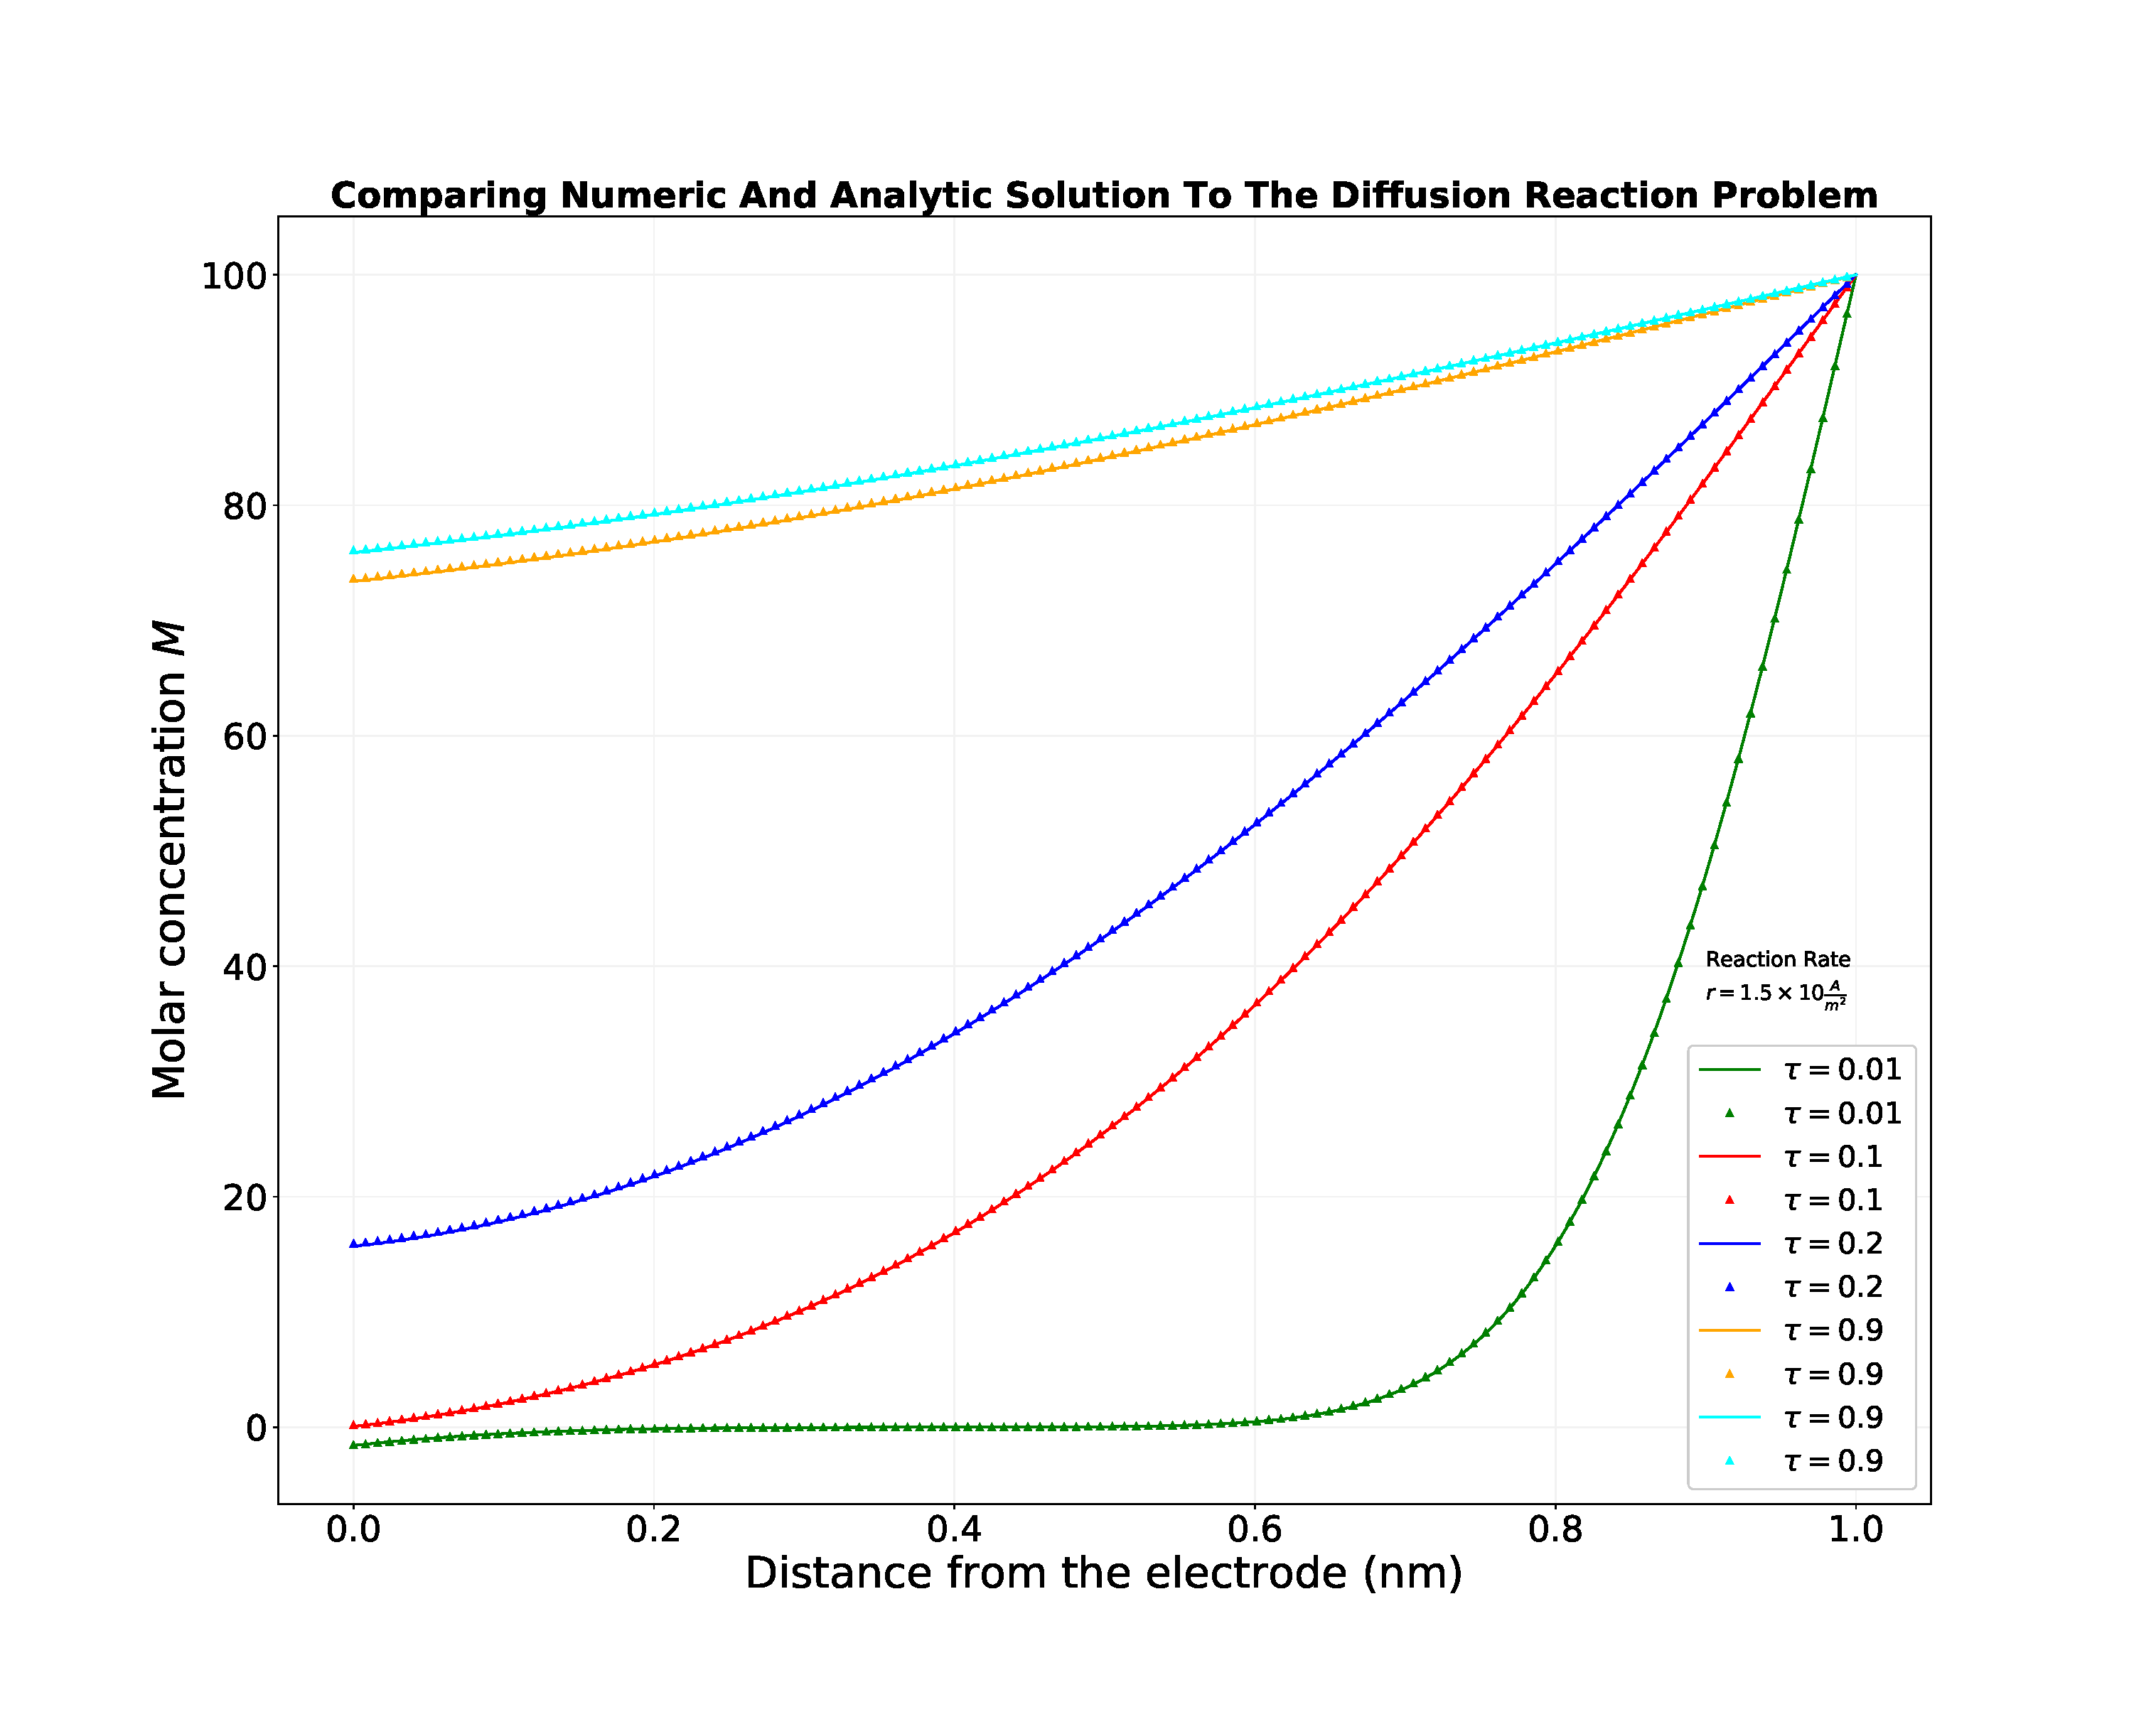
\includegraphics[width=\textwidth]{diffusion-reaction-comparison}
\caption{Concentration profiles at increasingly large $\tau$. The method only yields physically reasonable results for very small  current densities. This is due to the fact that we cannot impose current when there charge carriers. The effect is seen in the green curve ($\tau = 0.01$)}
\label{fig:diffusion-reaction-comparison}
\end{figure}

